\section{建模、扩展与跨求解器比较}
\label{chapter:04}

% block-id: auto.04.heading1
\hypertarget{auto.04.heading1}{}
\subsection{Wolfram 校准与模型扩展}

% block-id: auto.04.p1
\hypertarget{auto.04.p1}{}
归档的 rc.2 Wolfram 案例记录 MCP 初始化、工具发现和实际调用，并将解析计算、测试、图形及 Notebook 保存连接起来。单圆线基准在 200 kHz 下给出 Rac=\metric{q1_rac} mΩ/m、损耗 \metric{q1_loss} W/m；复电流积分与焦耳功率积分分别检验归一化及 RMS 约定。解析基准及原生 Notebook 的工具能力分别来自数学定义与 AgentTools 接口。\cite{BESSEL,AGENTTOOLS}

% block-id: auto.04.figure
\hypertarget{auto.04.figure}{}
\begin{figure*}[!htbp]
\centering
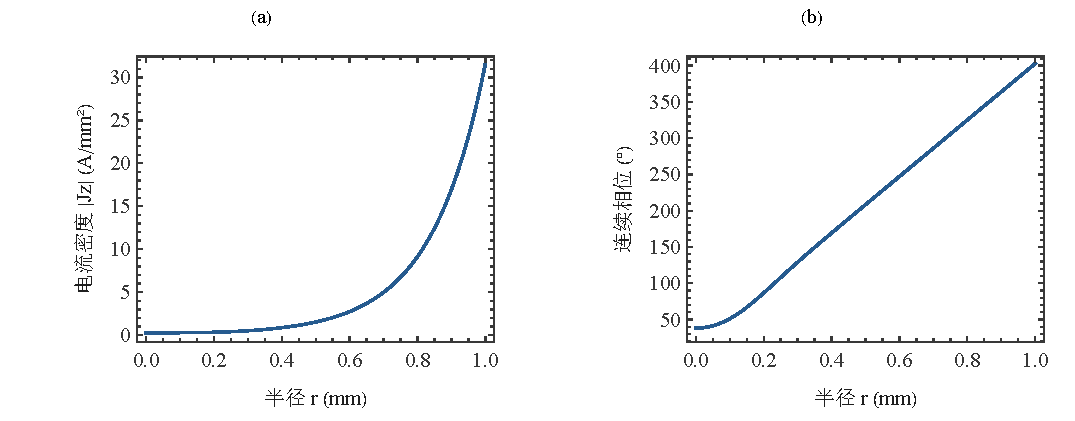
\includegraphics[width=\linewidth,height=.72\textheight,keepaspectratio]{../../assets/zh-CN/q1_profile.pdf}
\caption{单圆线径向电流幅值与相位。 铜导体直径 2 mm，200 kHz、20 A RMS。 (a) RMS 幅值；(b) 连续显示的相位。 相位显示采用径向连续提升，幅值保留 RMS 归一化。径向样本来自保存的 Bessel 解析数据。}
\label{fig:q1_profile}
\end{figure*}

% block-id: auto.04.p2
\hypertarget{auto.04.p2}{}
频率扩展案例将单频解析实现扩展为频率研究，保存源码差异、参数和新运行结果，并检验积分、低频极限及原单频回归。该案例说明智能体修改可以通过确定性检查进入研究流程；其验收范围是解析实现及所测频率条件，后续增加材料频散或热耦合时需建立相应物理检查。

% block-id: auto.04.heading2
\hypertarget{auto.04.heading2}{}
\subsection{Maxwell 建模、求解与交叉比较}

% block-id: auto.04.p3
\hypertarget{auto.04.p3}{}
Ansys 案例从运行器所属会话连接进入 MCP，完成小型七股 Maxwell 模型的材料、激励、求解和结果回读。rc2\_maxwell\_mcp\_verified\_01 及关联恢复运行通过端口与功率范围内的检查；协议探针自身的结果保留为协议状态。任务取消和新运行恢复另有独立记录，因而可以检查从任务身份到实际 AEDT 执行的对应关系。

% block-id: auto.04.p4
\hypertarget{auto.04.p4}{}
Wolfram 与 Maxwell 比较采用直线绝缘七股、共同端电压、总电流约束及受控铜回流。对齐项目包括股数、多边形截面、股径、回流内外半径、外域半径、轴向深度、频率和总电流。保存比较中的逐股复电流相对 L2 差异为 0.0106814\%，束内 Rac 相对差异为 0.00132823\%；相应电阻为 318.290316 和 318.294544 mΩ/轴向m。

% block-id: auto.04.p5
\hypertarget{auto.04.p5}{}
这些数值描述该案例的跨实现一致程度。两套实现使用独立网格和插值阶次，导体截面为 42 边形，回流分段也可能不同；Maxwell 使用一次自适应求解，尚未建立空间和边界收敛。案例铜面积小于 Q2 要求。因此，比较结果作为共同端口实现的交叉核查，进一步的精度估计需改变网格与边界并分析结果变化。
